% !TeX spellcheck = en_GB
\section{Introduction to Bayesian statistics}

\subsection{Bayesian basics}

The Bayesian approach is based on the idea, that a prior distribution of the data is assumed and the model is adjusted to this prior.

To perform a Bayesian Data Analyses the following things are required:
\begin{description}
	\tightlist
	\item[observed Data] The data you want to have conclusions from
	\item[generativer Model] to generate new data according to your prior
	\item[prior information] quantify the uncertainty of parameters in your model (i.e. by including prior information)
\end{description}

\subsubsection{Workflow for Binomial models}
\begin{enumerate}
	\tightlist
	\item Run $n$ simulations of possible $\theta$ using the prior distribution.
	\begin{lstlisting}
prior = runif(n)
	\end{lstlisting}
	\item Build a generative model, which simulates the model based on the prior distribution of $\theta$.
	\begin{lstlisting}
generativemodel = function(theta) {
	rbinom(1, nSamples, theta)
}
	\end{lstlisting}
	\item Simulate $n$ times using the generative model
	\begin{lstlisting}
simdata = rep(NA, n)
for(i in 1:n) {
	simdata[i] = generativemodel( prior[i] )
}
	\end{lstlisting}
	\item Calculate the posterior by checking which simulation resulted in the measured value(s)
	\begin{lstlisting}
posterior = prior[simdata == nSignedUp]
	\end{lstlisting}
\end{enumerate}

Step 2 and 3 can be made in one step, in case the generative model is as simple as in the shown example:
\begin{lstlisting}
simdata = rbinom(n, nSamples, prior)
\end{lstlisting}

\paragraph{Inference}
If a posterior is given, the following code snippets can be used for inference:
\begin{lstlisting}
mean(posterior) # the mean success rate
quantile(posterior, c(0.05, 0.95)) # the 90% confidence interval

# What's the probability of a success rate higher than x
sum(posterior[posterior>x])/length(posterior)

# If the experiment is repeated m samples, how big is the success rate
successForM <- rbinom(length(posterior), m, posterior)
\end{lstlisting}

\subsubsection{Possible prior distributions}

\paragraph{Uniform}
In case there is no knowledge about the distribution of $\theta$ the uniform distribution should be used. For the prior the uniform distribution must have its limits at 0 and 1.

\paragraph{Beta distribution}
\begin{gather*}
X\sim Beta(a, b)\\
E(X) = \frac{a}{a+b}\\
Var(X) = \frac{ab}{(a+b+1)(a+b^2)}\\
mode(X) = \frac{a-1}{a+b-2}
\end{gather*}

Mode = position of $f(x)_{max}$.

\begin{figure}[H]
	\centering
	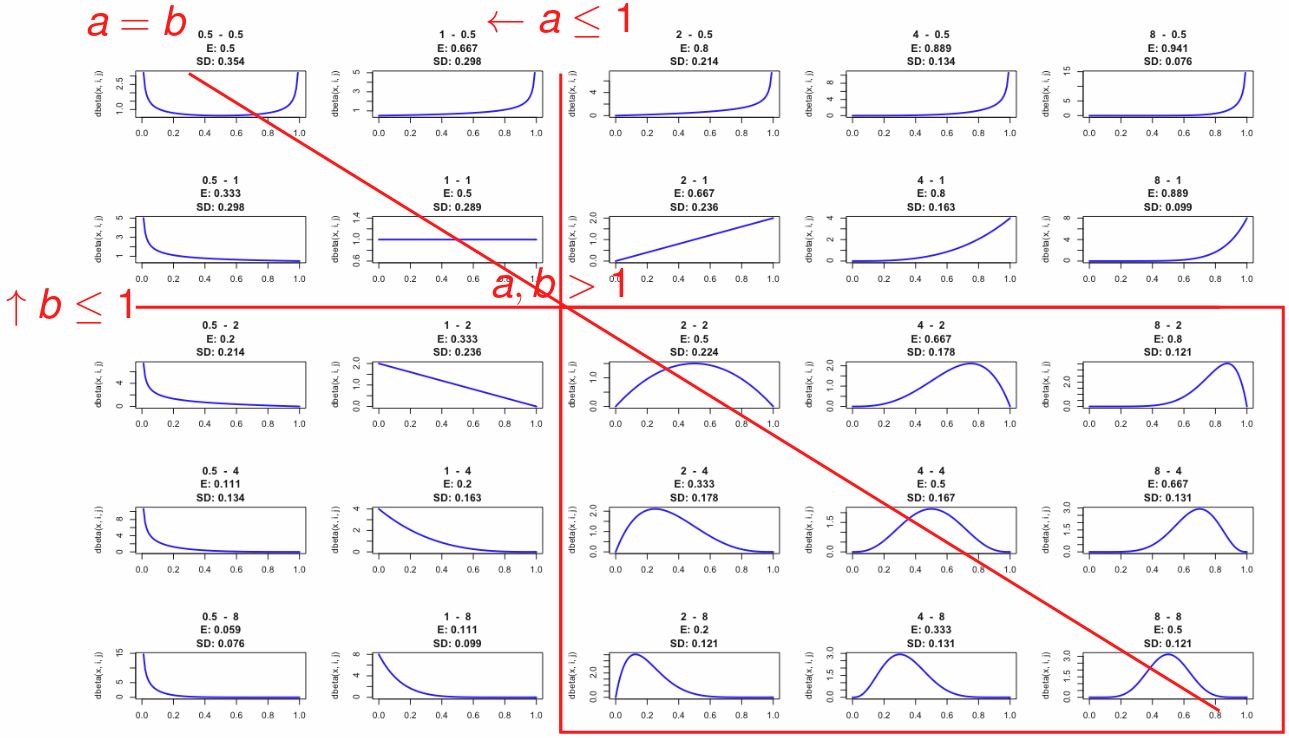
\includegraphics[width=\textwidth]{images/beta-examples.png}
	\caption{Examples of the beta distribution using different a and b values}
\end{figure}

\paragraph{Gamma distribution}
\begin{gather*}
X\sim Gamma(a, b)\\
E(X) = \frac{a}{b}\\
Var(X) = \frac{a}{b^2}\\
mode(X) = \frac{a-1}{b} (if \; a \geq 1)
\end{gather*}

\paragraph{Beta-binomial}
The Beta-binomial distribution is a Binomial distribution with N trials in which the probabilities of success are randomly drawn from a Beta(a, b) distribution.
\begin{gather*}
X\sim BetaBinom(N, a, b)\\
E(X) = N\frac{a}{a+b}\\
Var(X) = N\frac{ab}{(a+b)^2}\frac{a+b+N}{a+b+1}
\end{gather*}

\paragraph{Comparison with the frequentist approach}
Bayesian is an extension of the frequnetist approach. If not sure, start with a flat prior, the result is identical.

\subsection{Approximate Bayesian computation}
\subsubsection{Conditional probability}
\begin{gather*}
P(A|B) = \frac{P(A\cap B)}{P(B)}\\
P(A,B) = P(A|B)P(B) + P(B|A)P(A)\\
\Rightarrow P(A|B) = \frac{P(B|A)P(A)}{P(B)} = \frac{P(B|A)P(A)}{\sum_{i=1}^{n}P(B|A_i)P(A_i)}
\end{gather*}

For Bayesian modeling:
\begin{equation*}
P(\theta|D) = \frac{P(D|\theta)P(\theta)}{P(D)} = \frac{P(D|\theta)P(\theta)}{\sum_{i=1}^{n}P(D|\theta_i)P(\theta_i)} \propto P(D|\theta)P(\theta)
\end{equation*}

\subsubsection{Rejection algorithm}
Instead of throwing away all samples where the simulated data is not equal to the real data, one can set a small threshold $\epsilon$ to collect $||D_i-D||<\epsilon$ with $D$ as the Data and $D_i$ as simulated data. 

\subsection{A/B testing}
A/B testing is a way to compare two alternatives, typically by testing a subjects' response to variant A against variant B, and determining which of the two variant is more effective.

\mbox{}\\
This can be achieved by ``fitting'' two models and test the confidence intervals of parameter $\theta_A$ and $\theta_B$.

\begin{lstlisting}
A.prior = runif(n)
B.prior = runif(n)

A.sim = rbinom(n, numSamples, A.prior)
B.sim = rbinom(n, numSamples, B.prior)

ind = ((A.sim == A.success) & (B.sim == B.success))
A.posterior = A.prior[ind]
B.posterior = B.prior[ind]
\end{lstlisting}

\paragraph{Profit maximization}
Is a special case of A/B testing where one of the variants might be more effective but more expensive, too. In this case, the profit maximization can be calculated using $\theta$ and the expected gain.
\begin{equation*}
profit_i = \theta \cdot (income_i - cost_i)
\end{equation*}

\subsection{Discrete probability models}
Until now, we simulated and conditioned on observed data, to get a random sample from the posterior. A more analytical approach is to use a special prior distribution, which is called the \textbf{conjugate prior}.

\mbox{}\\
\textbf{Conjugate prior}: A prior distribution for a given generative model (a.k.a. likelihood function) which results in the same family for the posterior distribution.

\subsubsection{Binomial model}
The conjugate prior for the binomial model is the beta distribution.

\begin{equation*}
	L(\theta) = P(D|\theta) = {{n}\choose{s}}\theta^s(1-\theta)^{n-s}
\end{equation*}

With $L(\theta)$ as Likelihood, $n$ the number of trials and $s$ the number of success.

If the prior is beta distributed, the posterior will be beta distributed, too:
\begin{gather*}
\theta\sim Beta(a, b)\\
\theta|D\sim Beta(a+s, b+n-s)
\end{gather*}

=> The more samples, the lower the influence of the initial $a$ and $b$.

\subsubsection{Geometric distribution}
The geometric distribution takes values in $\mathbb{N}_0$. It represents the number of failures in a sequence of Bernoulli trials before a success occurs.
\begin{gather*}
P(X=n|\theta) = \theta(1-\theta)^n\\
E(X) = \frac{1-\theta}{\theta}\\
Var(X) = \frac{1-\theta}{\theta^2}
\end{gather*}

With a $Beta(a,b)$ distributed prior, the posterior distribution is:
\begin{gather*}
\theta|D\sim Beta(a+1, b+x) = Beta(a+1, b+\sum_{i=1}^{n}x_i)
\end{gather*}
With $x_i$ being the number of failures in experiment i before a success occurred.

\subsubsection{Poisson model}
This model counts the number of rare events in a fixed interval of time or space if these occur randomly and independent of each other with a constant rate.
\begin{gather*}
X\sim Pois(\lambda)\\
E(X) = \lambda\\
Var(X) = \lambda
\end{gather*}

The conjugate prior for the Poisson model is the Gamma distribution.
\begin{gather*}
\lambda \sim Gamma(a, b)\\
\lambda|D \sim Gamma(a+\sum_{i=1}^{n}x_i, b+n)
\end{gather*}
With $x_i$ being the number of events within the $i$th period and $n$ the number of periods.

\subsubsection{Hypergeometric distribution}
Basically the binomial distribution without replacement. It represents the number of $m$ success in $n$ draws without replacement from a set of size $N$ containing exactly $M$ objects with a certain feature.
\begin{gather*}
X\sim HyperGeo(n,N,M)\\
P(X=m|n, N, M) = \frac{{{M}\choose{m}}{{N-M}\choose{n-m}}}{{N\choose n}}\\
E(X) = n\frac{M}{N}\\
Var(X) = n\frac{M}{N}\frac{N-M}{N}\frac{N-n}{N-1}
\end{gather*}

With a Beta-binomial prior on M i.e. $M\sim BetaBin(N, a, b)$ the posterior distribution of M is:
\begin{equation*}
M-m\sim BetaBin(N-n, a+m, b+n-m)
\end{equation*}